\documentclass[11pt,a4paper]{report}
\usepackage[utf8]{inputenc}
\usepackage[T1]{fontenc}
\usepackage{amsmath}
\usepackage{amsfonts}
\usepackage{amssymb}
\usepackage{graphicx}
\usepackage{float}
\usepackage{cleveref}

\newcommand{\dd}{\mathrm{d}}

\usepackage[a4paper, total={7in, 9.5in}]{geometry}

\begin{document}

\begin{center} 
\textbf{Assignment 2} 
\end{center}

In this assignment, we will solve for the temperature in a metal bar which is fixed at temperature $T_0 = 0$ degrees (Celsius) at the left end and $T_L = 100$ degrees (Celsius) at the right end.  

We can assume that temperature $T$ is only a function of x-coordinate along the bar, i.e., $T = T(x)$, and with this and the other simplifying assumptions, we get the following second-order Ordinary Differential Equation for $T$:
\begin{equation}\label{eq:ode}
-\kappa A \frac{\dd^2 T(x)}{\dd x^2} = A q_{ext}(x), \qquad \text{for all } 0 \leq x \leq L .
\end{equation}
The boundary conditions are
\begin{equation}\label{eq:bc}
T(x=0) = T(0) = T_0, \qquad T(x=L) = T(L) = T_L .
\end{equation}
Here, $A$ is the area of the cross-section of the bar (we assume that the shape and size of the cross-section is same throughout the length, see \cref{fig:bar}), $\kappa > 0 $ a positive constant (from Fourier's law) referred to as heat conductivity, $q_{ext}  =q_{ext}(x)$ external heat supplied at $x$, $L$ is the length of the bar. 

\begin{figure}[H]
\centering
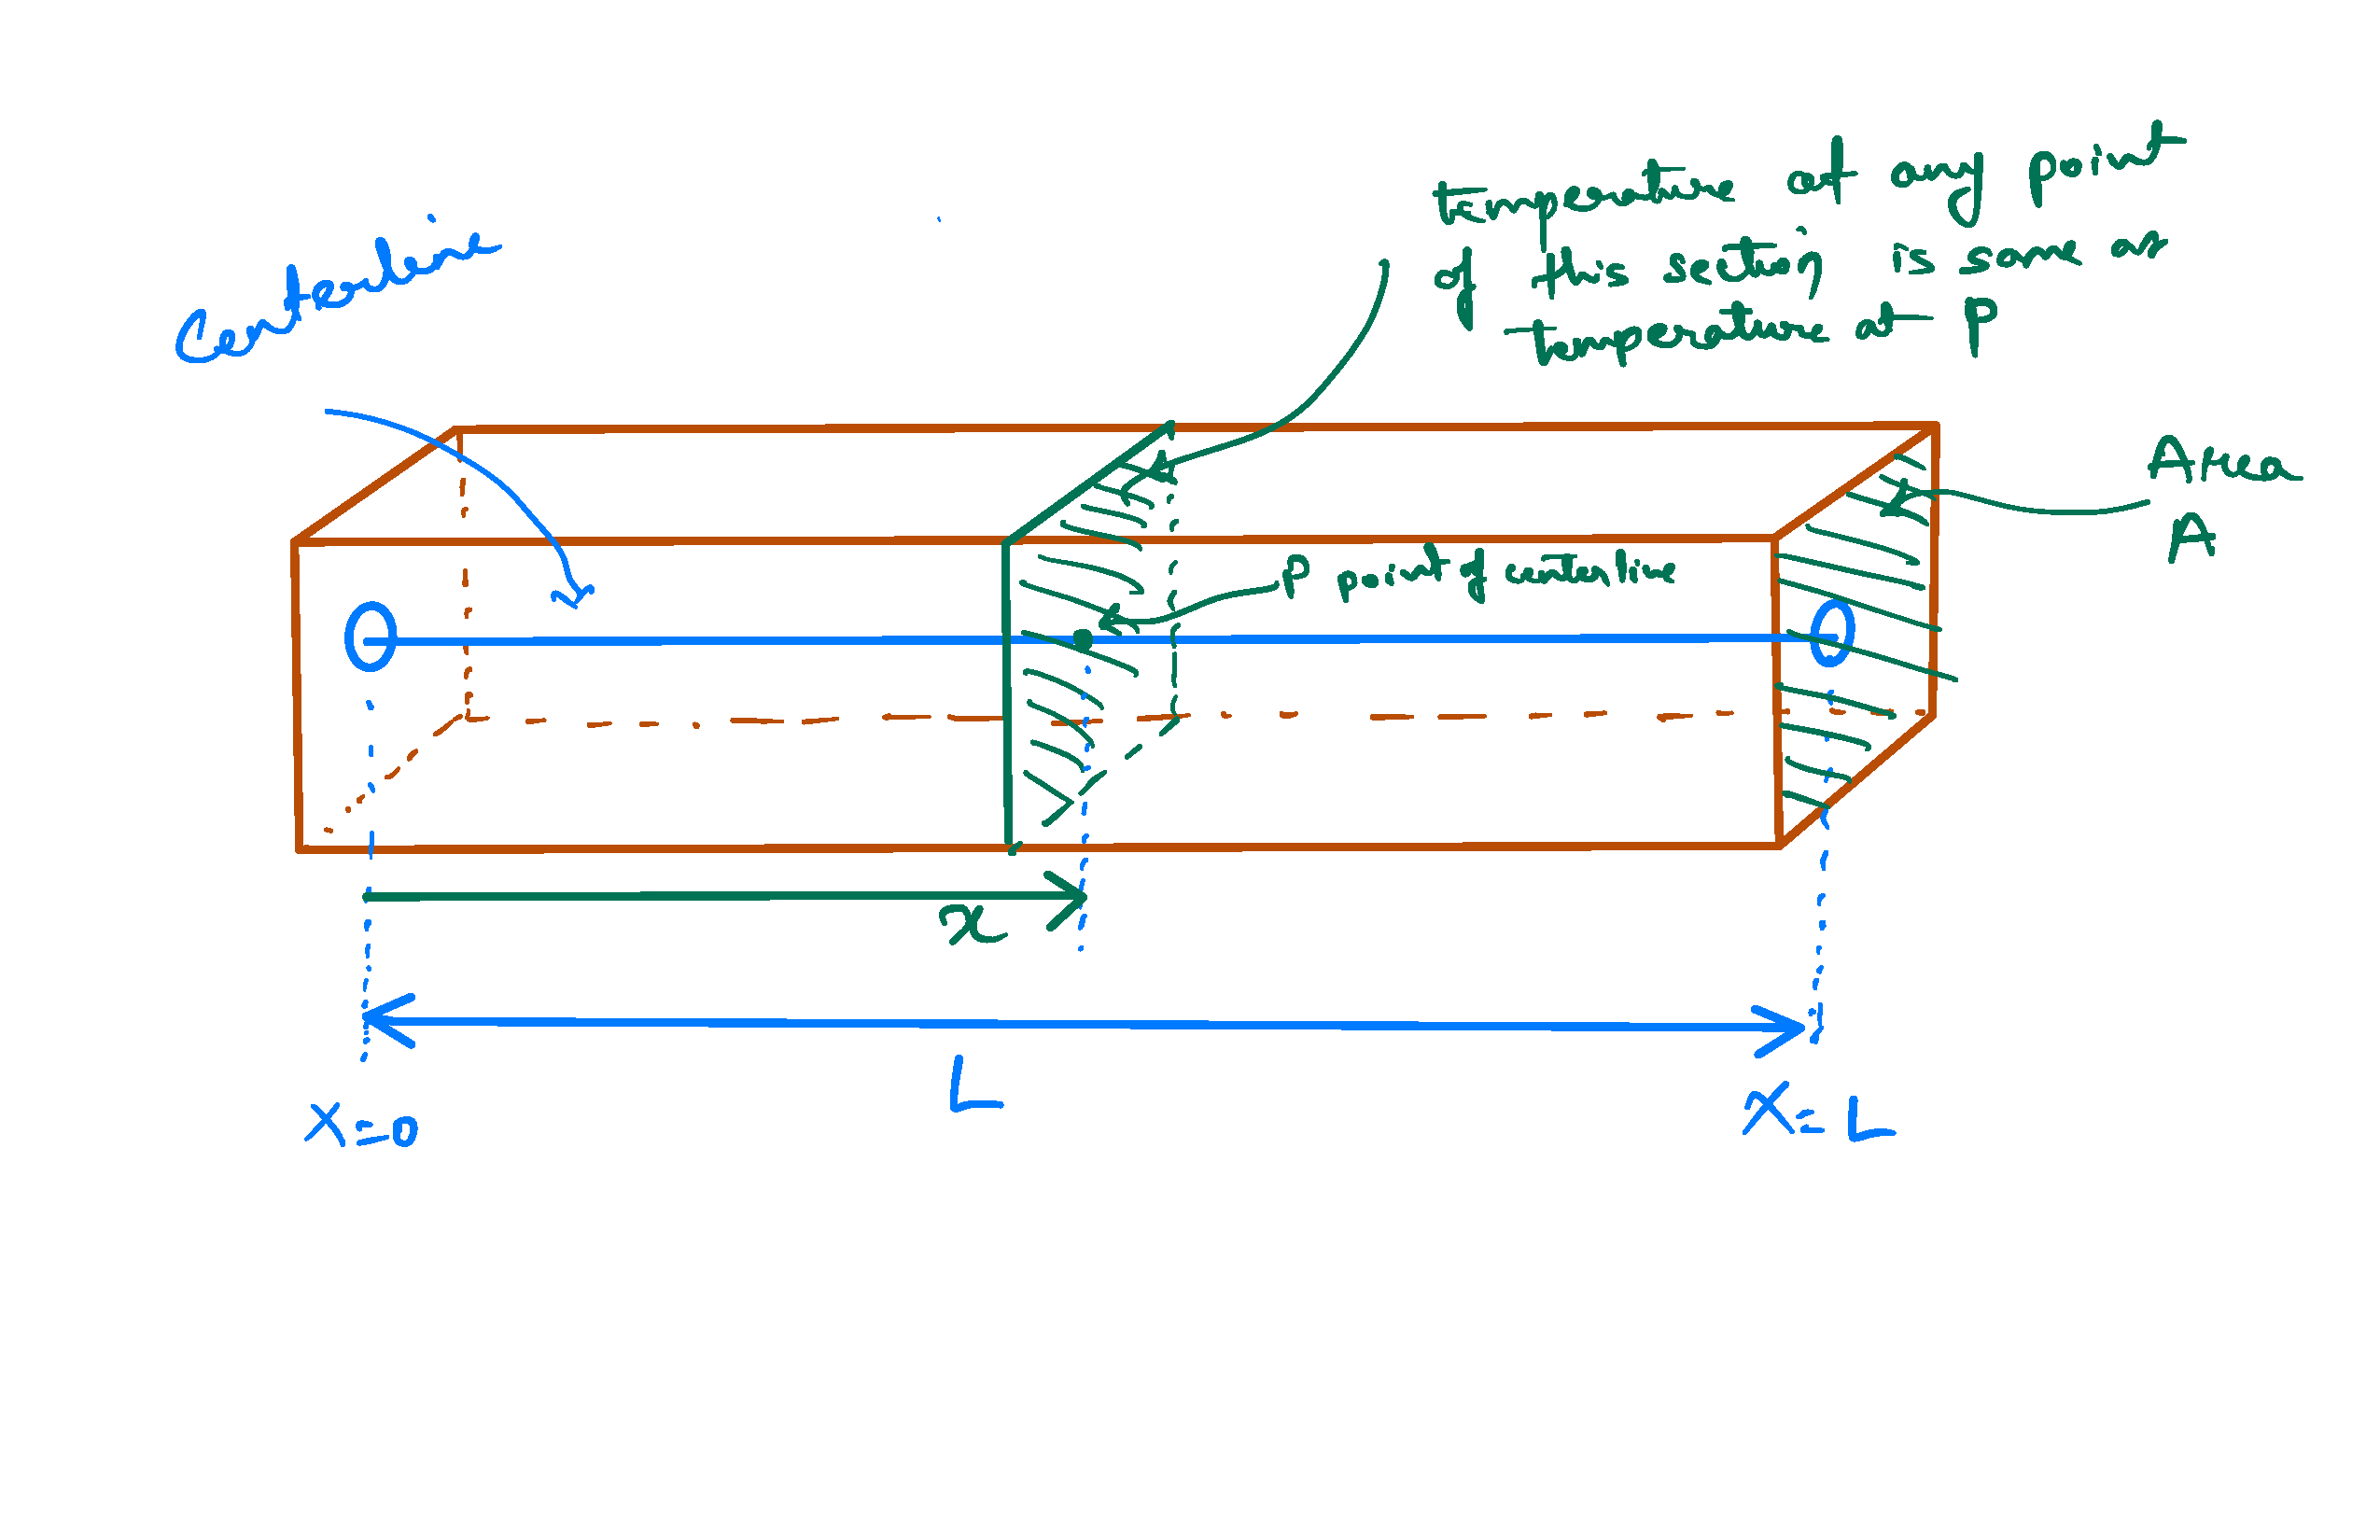
\includegraphics[width=0.9\textwidth]{Draw Bar.pdf}
\caption{Thermal heating of the bar with a uniform cross-section.}\label{fig:bar}
\end{figure}

\vspace{10pt}
\noindent\textit{Remark 1.} See the supplementary file `A2\_heating\_bar.pdf' for the derivation.

\vspace{10pt}
\noindent\textit{Parameters.} Let $L = 1$ m, $A = 1$ m$^2$, $T_0 = 0$ Celsius, $T_L = 100$ Celsius, and $\kappa = 1/200$ Watts/$(\text{m} \times \text{Celsius})$. Further, fix external heat function (in units of Watt/$(\text{m}^3$) as follows:
\begin{equation}\label{eq:qext}
q_{ext}(x) = 12x^2 + \cos(5x) + 100x \sin(10x).
\end{equation}

\vspace{10pt}
\noindent\textit{Remark 2.} Read carefully the problems. They all are easy and results can be verified by just plotting the temperature in matlab and observing it. I have also included the hints in the file `A2\_hints.pdf'. Before you panic (I hope not!!), do check the hints; some problems are practically solved in the hints file.   

\vspace{10pt}
\noindent\textbf{Problem 1 (10 marks).} \textit{Exact solution} of \eqref{eq:ode} with boundary conditions \eqref{eq:bc} is given by
\begin{equation}
T(x) = T_0 + \left[ \frac{T_L - T_0 + \frac{1}{\kappa} Q_2(L)}{L} \right] x - \frac{1}{\kappa} Q_2(x), \qquad \text{for } x \in [0, L],
\end{equation}
where $Q_2 = Q_2(x)$ is a function of $x$ and is given by
\begin{equation}
Q_2(x) = \int_{0}^x Q_1(y) \dd y.
\end{equation}
And, finally $Q_1$ function is defined as
\begin{equation}
Q_1(x) = \int_0^x q_{ext}(y) \dd y.
\end{equation}

\begin{itemize}
\item[(i)] For $q_{ext}$ given in \eqref{eq:qext} and the parameter values specified earlier, verify that 
\begin{align}\label{eq:sol}
Q_1(x) &= 4 x^3 + \frac{\sin(5x)}{5} + \sin(10x) + 10x\left(2 \sin^2(5x) - 1\right), \notag \\
Q_2(x) &= x^4 - x \sin(10x) - \frac{2 \cos^2(5x)}{5} - \frac{\cos(5x)}{25} + \frac{11}{25}.
\end{align}

With the exact formula for $Q_1$ and $Q_2$, the temperature function is simply (note this function as it will be used in all problems below!)
\begin{equation}\label{eq:exactT}
T(x) = 100 x + 200 x Q_2(1) - 200 Q_2(x) .
\end{equation}

\noindent\textit{Remark 3.} In the hints file, I show how you can verify formulas for $Q_1$ and $Q_2$ using MATLAB symbolic library. Use the codes in the hints file to complete this problem.

\item[(ii)] Plot $q_{ext}$ and $T$ ($T$ is given by \eqref{eq:exactT}) in the same plot. Also plot the horizontal lines $y = 80$ and $y= 40$ in the same plot. Add labels to each curves in MATLAB plot. (See hints file where all this is practically done. Try to make new changes to the codes I provide as you see fit.)

\item[(iii)] \textit{(Optional)} Show that $T$ in \eqref{eq:exactT} satisfies ODE \eqref{eq:ode} and boundary conditions \eqref{eq:bc}. That is, compute $-\kappa A\frac{\dd^2 T}{\dd x^2}$ and show that it is equal to $A q_{ext}$, and show $T(0)$ and $T(1)$ is equal to $T_0$ and $T_1$, respectively.

\end{itemize}

\vspace{10pt}
\noindent\textbf{Problem 2 (25 marks).} \textit{Roots problem}. Find a point in the bar, i.e. $x$, such that the temperature $T(x)$ is 80 Celsius. I.e., solve roots problem $f(x) = 0$ with $f(x) = T(x) - 80$, where $T$ is given by \eqref{eq:exactT}. 
\begin{itemize}
  \item[(i)] Use \textbf{incremental search method} with $n  = 5$ intervals and initial bracket $[0,1]$, and find the interval $[x_l, x_u]$ that contains the root of function $f(x) = T(x) - 80$. 
  
  \item[(ii)] With interval $[x_l, x_u]$ computed in (i) above, now apply \textbf{Bisection method} to more accurately locate the root of function $f(x) = T(x) - 80$. For Bisection method, set max iteration to 100 and tolerance on relative percentage error of $0.001\%$ . 
\end{itemize}

\noindent\textit{Remark 4.} Using the plot in \textbf{Problem 1}, you can verify your results. This works also for the \textbf{Problems 3 and 4}.

\vspace{10pt}
\noindent\textbf{Problem 3 (25 marks).} \textit{Roots problem}. Find a point in the bar, i.e. $x$, such that the temperature $T(x)$ is 40 Celsius. I.e., solve the roots problem $f(x) = 0$ with $f(x) = T(x) - 40$. 
\begin{itemize}
  \item[(i)] With initial guess $x_0 = 0.15$, apply the \textbf{Newton-Raphson method} to solve the roots problem $f(x) = T(x) - 40 = 0$. Use max iteration $100$ and tolerance of relative percentage error $0.001\%$.
  
  \item[(ii)] With initial guess $x_0 = 0.15$, apply the \textbf{Secant's method} with max iteration $100$ and tolerance of relative percentage error $0.001\%$. For the Secant's method, use $h=0.0001$ in approximation of a derivative.
\end{itemize}

\vspace{10pt}
\noindent\textbf{Problem 4 (40 marks).} \textit{Optimization problem}. It is important to know what is the maximum temperature in the bar. Therefore, solve the following maximization (optimization) problem:
\begin{equation}
  \max_{x\in [0.6,0.9]} T(x).
\end{equation}
In the above, I could also have $x \in [0,1]$, but judging by the plots in \textbf{Problem 1}, I know that the maximum is somewhere in this interval $[0.6, 0.9]$ so we are good. Complete this problem in the following steps:

\begin{itemize}
  \item[(i)] We know that at points where the function is maximum or minimum, the derivative of a function will be zero. I.e., if at $\bar{x}$, $T(\bar{x})$ is maximum, then $\dd T (\bar{x})/\dd x = 0$. We use this fact to convert the maximization problem into  the roots problem: Let $f(x) = \dd T(x) / \dd x$, then find $\bar{x}$ in the interval $[0.6, 0.9]$ such that $f(\bar{x}) = 0$. Use the \textbf{Bisection method} with the max iterations 100 and error (relative percentage error) tolerance $0.001\%$. Of course, for the Bisection method, use  initial bracket $[0.6, 0.9]$, i.e., $x_l = 0.6$ and $x_u = 0.9$. Also, report the value of temperature $T$ at the approximate solution $\bar{x}$ from the Bisection method. 

\item[(ii)] Repeat (i)  but now using the \textbf{Secant's method} with the initial guess as $x_0 = 0.7$. As before, use $h = 0.0001$ to compute the approximate derivatives in the Secant's method. 
\end{itemize}

\end{document}